Un BDMS può essere diviso in 3 livelli, dal più alto (astratto) al più basso (rappresentazione dei dati concreti):
\begin{center}
    Viste\\
    Livello Logico\\
    Livello Fisico
\end{center}
Il DBMS \`e composto da vari parti, che a loro volta sono suddivise in moduli/gestori.
\begin{itemize}
    \item Query Manager
    \begin{itemize}
        \item Gestore degli accessi
        \item Gestore dell'integrità
        \item Elaboratore delle interrogazioni
    \end{itemize}
    
    \item Transaction Manager
    \begin{itemize}
        \item Gestore della concorrenza
        \item Gestore del ripristino
    \end{itemize}
    
    \item Gestore delle strutture di memorizzazione
\end{itemize}

\begin{figure}[h]
    \centering
    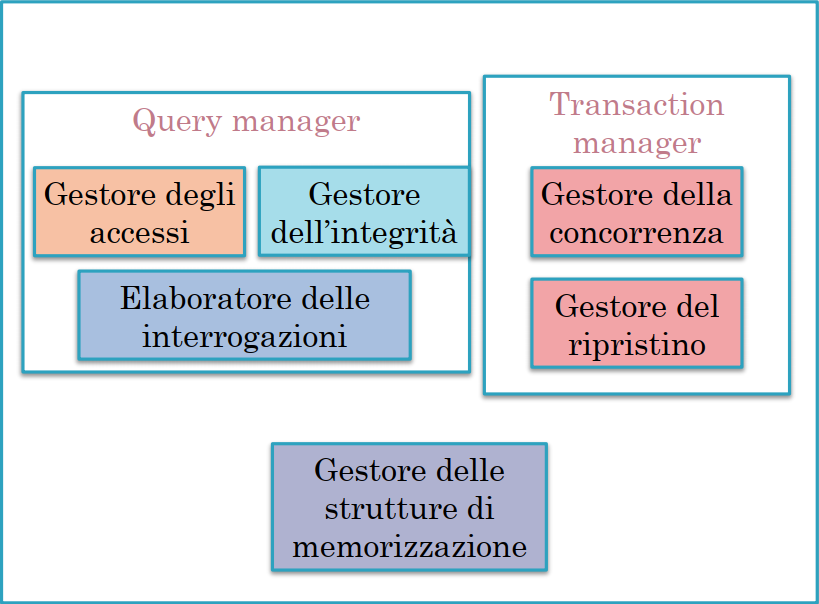
\includegraphics[width=0.8\textwidth, keepaspectratio]{componentiDBMS.png}
    \label{fig:componentiDBMS}
\end{figure}